\section{Tools}
\label{chap:ch3}

For this verification assignment, two tools were used to ensure the reliability and safety of ACAS XU: alpha-beta-CROWN and nnenum. Alpha Beta Crown serves as a neural network verifier based on an efficient linear bound propagation framework, built on  bound-propagation-based neural network verifiers: CROWN \cite{xu2020automatic, zhang2018efficient}, alpha-CROWN \cite{xu2021fast}, beta-CROWN \cite{wang2021beta}, GCP-CROWN \cite{zhang2022general}, and nonlinear branch-and-bound \cite{shi2023generalnonlinear}. Nnenum is a verifier that relies on multiple levels of abstraction to achieve high performance  verification of ReLU networks without sacrificing completeness \cite{10.1007/978-3-030-76384-8_2}. In the following sections, the setup of these tools is presented.

\subsection{Alpha-Beta-CROWN}

Setting it up involved a two-step process: first, installing Miniconda and then the tool itself. There were no complications in the first part, as there is an executable file available on their official site that takes care of the entire setup once run. However, the latter part, involving the tool's installation, presented numerous complications.

The setup of Alpha Beta Crown followed their "Installation and Setup" section outlined on GitHub. The first command was supposed to clone their GitHub repository including "auto\_LiRPA"\cite{xu2020automatic}, an essential component for the tool's functionality. Despite running this command, only the tool's files were retrieved due to permission denials that restricted access to the second GitHub repository. Resolving this required an additional step: manually obtaining the missing necessary files and placing them in their indicated location. The next phase involved creating the conda environment using the specified command, which led to an error that can be observed in figure \ref{Fig_Err}. 

\begin{figure}[htbp]
	\centering
		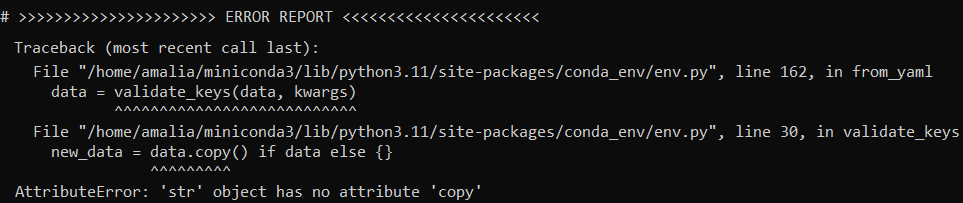
\includegraphics[width=14cm]{./Figures/ToolErr.png}
	\caption{Creating conda environment error}
	\label{Fig_Err}
\end{figure}

\par This error consumed a considerable amount of time, as the error message initially suggested an issue with the script. After extensive investigation, the root cause was traced to the configuration file. Instead of containing the necessary configuration for the conda environment, it referenced another configuration file by name. After resolving the configuration file issue, the installation of the tool seemed successful. However, when attempting to run it, another problem emerged indicating a missing library, "auto\_LiRPA". Although the necessary files existed, the error message revealed a discrepancy in the file path. It seemed that the correct location for this library was wrongly specified. With this adjustment, the setup concluded, and the tool run successfully.

\subsection{Nnenum}

As a prerequisite, the tool required Docker to be installed, which simplified the process by eliminating all dependencies challenges thanks to the docker container properties. The setup followed their "Getting started" section outlined in Github. For the actual installation of the tool the GitHub repository needs to be cloned. There are two commands that needs to be run in order for the tool to work. The first one is for building the image and the second one is for getting the shell after building the image. Both commands are in the docker file present in the tool repository.

\par If both commands run successfully the tool is installed and running, ready to be used. To double check if the tool is running the container should be visible in the docker desktop application, which can be observed in figure \ref{Fig_NneumRunning}. The installation of the tool was simple and did not produce any error or unexpected behavior.

\begin{figure}[htbp]
	\centering
		
\includegraphics[width=15cm]{./Figures/nnenumRunning.png}
	\caption{Nnenum container running}
	\label{Fig_NneumRunning}
\end{figure}